\section{The GEANT4 Model of the XENON100 Detector}
\label{secGeant4model}

A detailed model of the XENON100 detector has been created with the GEANT4 toolkit~\cite{g4}.
The schematics are shown in Fig.~\ref{figDetectorModel}, the water tanks around the shield box and the polyethylene slab on the bottom are not included. The model has been extensively used for  Monte Carlo simulations of light detection within the detector volume, of the response of the detector to various types of particles, and for predictions of the electronic recoil (Chapter~\ref{chERbackground}) and nuclear recoil (Chapter~\ref{chNRbackground}) backgrounds.

\begin{figure}[!ht]
\centering
\subfigure[]{
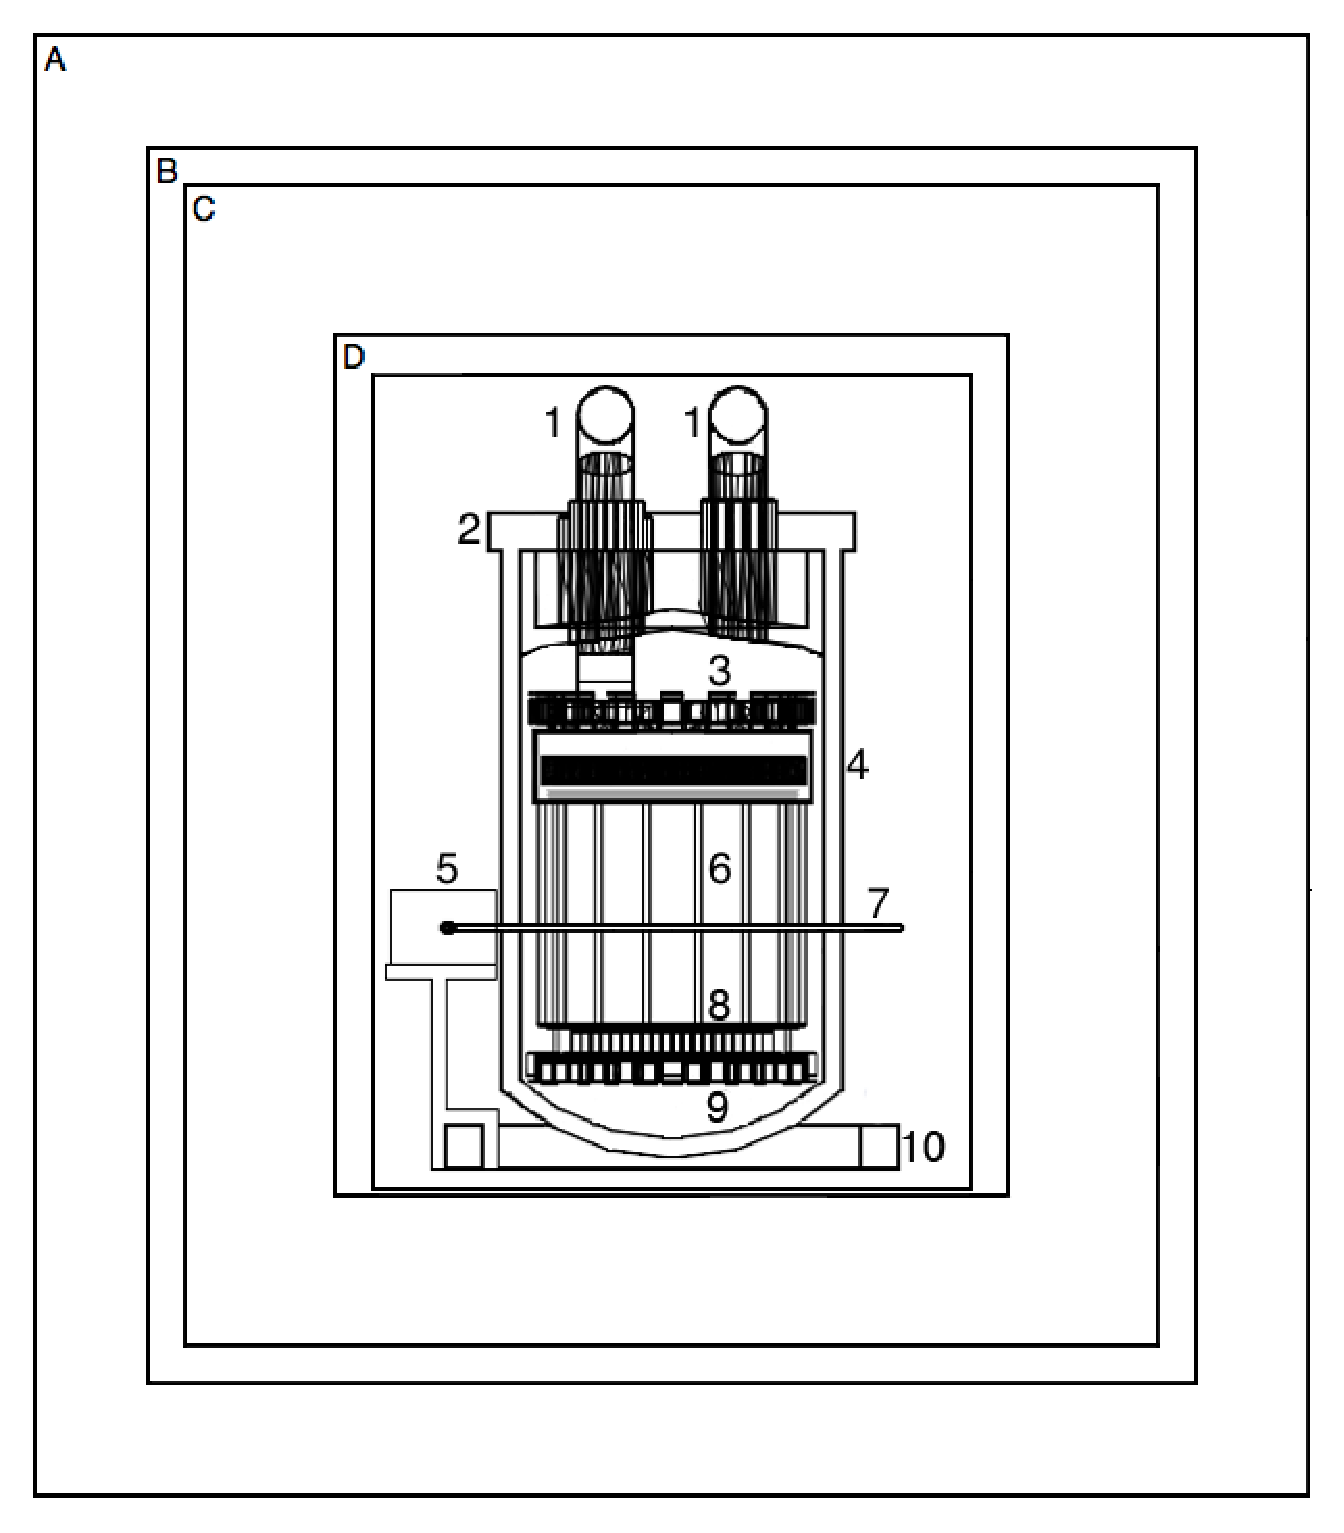
\includegraphics[height=0.5\linewidth]{plots/Geant4model/DetectorModel_shield_withLabels1.eps}
\label{figDetectorModel_1}}
\subfigure[]{
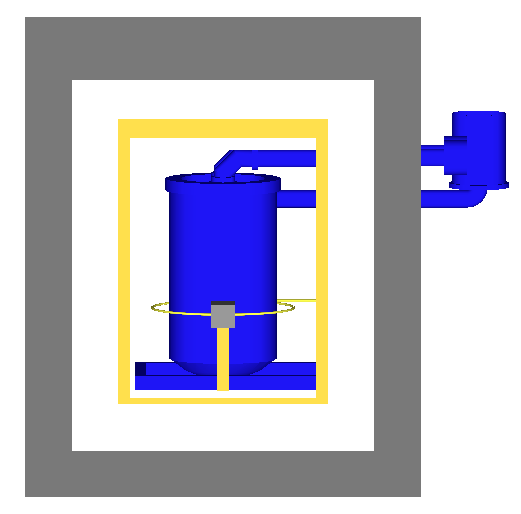
\includegraphics[height=0.51\linewidth]{plots/Geant4model/DetModel_withPTR.png}
\label{figDetectorModel_2}}
\caption[The GEANT4 model of the XENON100 detector and its shield]{The GEANT4 model of the XENON100 detector and its shield: A - outer lead layer, B - inner lead layer with low $^{210}$Pb contamination, C - polyethylene shield, D - copper shield; 1 -  pipes to the PMT feedthroughs and pumping ports, 2 - stainless steel cryostat, 3 - top and upper side veto PMT arrays, 4 - top PMT array in the TPC, in the gas phase inside the `diving bell', 5 - lead brick for calibration with $^{241}$Am-Be neutron source, 6 - TPC wall (PTFE panels), 7 - copper pipe for calibration sources, 8 - bottom PMT array in the TPC, 9 - bottom and lower side veto PMT arrays, 10 - support bars for the cryostat. 
The water shield and an additional polyethylene layer on the bottom are not shown. Figure (a) published in Ref.~\cite{EMBG}.}
\label{figDetectorModel}
\end{figure}

\begin{table}[!ht]
\centering
{\caption{Materials used in the XENON100 experiment, and their properties used in detector  modeling and background predictions}
\label{tabDetectorMaterials}
%\vspace{0.2cm}
\begin{tabular}{>{\footnotesize}l|>{\footnotesize}c|>{\footnotesize}l}
%\begin{tabular}{l | c | l}
\hline
Component 						& Density  			& Chemical composition  \\
								& [g/cm$^{3}$]			& \\
\hline
316Ti stainless steel					& 8.00 		& C 0.08\%, Si 1\%, Mn 2\%, P 0.045\%, S 0.03\%, \\
								&			& Ni 12\%, Cr 17\%, Mo 2.5\%, Ti 4.0\%, Fe 64.945\% \\
PTFE							& 2.20 		& -CF$_{2}$- \\
Copper							& 8.92 		& Cu 100\% \\
$Kovar$ metal						& 8.33 		& Fe 55\%, Ni 29\%, Co 16\%;  \\
Stainless steel						& 7.64 		& Fe 70\%, C 0.1\%, Si 0.5\%, Mn 0.7\%, \\
								& 	 		& Mn 0.7\%, Ni 8.6\%, Cr 18.3\% \\
Synthetic silica						& 2.20 		& SiO$_{2}$ \\
Borosilicate glass					& 2.21 		& SiO$_{2}$ 67.0\%, Al$_{2}$O$_{3}$ 4.3\%, B$_{2}$O$_{3}$ 18.0\%, \\
								&			& Li$_{2}$O 1.0\%, Na$_{2}$O 6.0\%, BaO 2.0\% \\
Aluminum	 (0.1~g/PMT)				& 2.70 		& Al 100\% \\
$Cirlex$							& 1.43 	 	& C$_{22}$H$_{10}$N$_{2}$O$_{5}$ \\
Ceramics							& 1.00		& NaAlSiO$_{2}$ \\
Polyethylene						& 0.92		& -CH$_{2}$- \\
Lead								& 11.34		& Pb 100\% \\
\hline
\end{tabular}
}
\end{table}

The main materials used in the detector model are listed in Table~\ref{tabDetectorMaterials}, together with their density and  chemical composition. Table~\ref{tabDetectorComponents} shows the total weight of detector and shield components, computed from the model and in agreement with the actual detector.



\begin{table}[!h]
\centering
\caption[Components and materials of the XENON100 detector and its shield]{Components and materials of the XENON100 detector and its shield. The total weight of the materials has been calculated with the GEANT4 model.  The cryostat vessels with the top flange and pipes, and the diving bell system are made from the grade 316Ti stainless steel and shown as one unit. The resistive voltage divider network for the TPC drift field is simplified in the model with a thin tube.}
\label{tabDetectorComponents}
%\vspace{0.2cm}
\begin{tabular}{>{\footnotesize}l |>{\footnotesize} r}
%\begin{tabular}{l|r}
\hline
Component 					& Amount of material  \\
\hline
Cryostat and diving bell (316Ti SS) & 73.61 kg 	\\
Support bars (316Ti SS) 			& 49.68 kg 	\\
Detector PTFE 					& 11.86 kg	\\
Detector copper 				& 3.88 kg 		\\
PMTs						& 242 pieces 	\\
PMT bases 					& 242 pieces 	\\
TPC resistor chain 				& 1.5$\times$10$^{-3}$ kg \\
Bottom electrodes (316Ti SS) 		& 0.23 kg 		\\
Top electrodes (316Ti SS) 		& 0.24 kg 		\\
PMT cables					& 1.80 kg 		\\
Copper shield 					& 2.1$\times$10$^{3}$~kg 	\\ 
Polyethylene shield 				& 1.6$\times$10$^{3}$ kg 	\\
Lead shield  (inner layer) 			& 6.6$\times$10$^{3}$ kg 	\\
Lead shield (outer layer) 			& 27.2$\times$10$^{3}$ kg 	\\
\hline
\end{tabular}
\end{table}

In the GEANT4 model, a PMT is simplified with a stainless steel case and a synthetic silica window inside a thin aluminum ring. The ceramic insulator and ZrAl getter are not included due to their low mass (Table~\ref{tabPMTmassModel}). The {\it Cirlex} base for the voltage divider network is approximated as a homogenous unit. 
For background predictions, only the 316Ti SS support rings for the mesh electrodes are considered in the model, given that the meshes are $\sim$100~$\mu$m thick and have a very low mass, leading to a negligible background from their radioactivity. For the photon propagation, the electrode meshes are implemented as 130~$\mu$m thick disks with the appropriate optical transparency.

By default, the entire decay chain simulated with GEANT4 is written into one event, as well as secondary particles, and this leads to pile-up of the energy depositions, and therefore wrong energy spectrum. A custom `G4StackingManagerAction' has been implemented in the XENON100 simulations, which postpones daughter decays to the next event. The total energy deposition for each event is calculated by summing up energy deposited by all primary and secondary particles, which is done separately for the target volume and for the veto. 

For the calculation of the final background rate in the Monte Carlo simulations, multiple scatter events are rejected taking into account the finite position resolution of the detector.  
A multiple scatter event is considered as a single scatter event if the interactions happen less than 3~mm apart in $Z$ (see Section~\ref{secPositionResolution}). This position resolution is given by the width of the S2 signals and the peak separation efficiency of the S2 peak finder algorithm.

%`
